\section{Preliminary Results}\label{sec:results}
All runs use the authors' MICA code (commit 54fae81) on the processed inputs they released, so differences from the paper do not come from our preprocessing. Our own implementation of the MICA distance matches theirs to within $10^{-6}$ on about 10,000 random Zeisel cell pairs and on 2,000 edges of MICA's saved PBMC14K graph, and we use it for the neighbor search.

\begin{table}[t]
\centering
\caption{MICA and PCA + Leiden on the authors' released inputs with all genes, scored by ARI under the paper's rule, where the true number of types is given and the labels pick the setting.}
\label{tab:repro}
\footnotesize
\setlength{\tabcolsep}{3.5pt}
\begin{tabular}{lrcccc}
\toprule
 & & \multicolumn{2}{c}{MICA} & \multicolumn{2}{c}{PCA + Leiden} \\
\cmidrule(lr){3-4}\cmidrule(lr){5-6}
Dataset & Cells & paper & ours & paper & ours \\
\midrule
Yan & 124 & 0.939 & 0.939 & 0.839 & 0.789 \\
Goolam & 124 & 0.544 & 0.544 & 0.572 & 0.308 \\
Buettner & 182 & 0.934 & 0.934 & 0.277 & 0.268 \\
Pollen & 249 & 0.942 & 0.951 & 0.874 & 0.858 \\
Chung & 317 & 0.655 & 0.655 & 0.170 & 0.319 \\
Usoskin & 622 & 0.847 & 0.835 & 0.860 & 0.598 \\
Kolodziejczyk & 704 & 1.000 & 0.727$^\ast$ & 0.996 & 0.564 \\
Klein & 2,717 & 0.980 & 0.980 & 0.820 & 0.977 \\
Zeisel & 2,903 & 0.744 & 0.714$^\ddagger$ & 0.630 & 0.839 \\
PBMC14K & 13,605 & 0.853 & 0.854$^\dagger$ & 0.754 & 0.878 \\
\bottomrule
\end{tabular}
\\[2pt]
\parbox{\columnwidth}{\scriptsize As in the paper, sets of up to 5,000 cells use MICA's small-data mode, where we give the final $k$-means 100 restarts and report the mean of three seeds, and PBMC14K uses graph mode. $^\dagger$Median of six runs, 0.850 to 0.857. $^\ddagger$Graph mode gives 0.755 to 0.781 over six runs. $^\ast$Not reproduced from the released files (Sec.~\ref{sec:results}). The paper's PCA + Leiden is Scanpy on 2,000 variable genes. Ours uses all genes, like MICA, and we report the median of three seeds.}
\end{table}


\subsection{Reproduction}
MICA comes within 0.05 of the published ARI on 9 of 10 datasets (Table~\ref{tab:repro}), and within 0.001 on six of them. In small-data mode MICA ends with one $k$-means call, and its default 10 restarts often stop at a worse optimum (on Chung, 0.589 against the published 0.655). On five sets the published score is that of the best fit, which 100 restarts usually reach, while on Pollen the best fit scores 0.980 against 0.942. On Zeisel our small-data run gives 0.714 against the published 0.744, and graph mode, which the authors' analysis scripts also ran, gives 0.755 to 0.781. Kolodziejczyk does not reproduce. MICA scores 0.727 on the released input, as in the authors' own notebook, so their 1.0 seems to come from an unreleased input.

The table also exposes a confound. Scanpy got 2,000 variable genes and MICA all genes, and the paper notes that Scanpy rose on PBMC14K from 0.69 with 1,000 genes to 0.82 with 3,000. Given all genes, Leiden reaches 0.878 on PBMC14K and 0.839 on Zeisel, ahead of MICA on both. On the other eight sets MICA stays ahead or level (mean ARI 0.82 against 0.59). With 2,000 matched variable genes, Leiden stays ahead on PBMC14K but falls behind MICA on Zeisel (0.66 to 0.74 against 0.76 to 0.81), so the gene set matters about as much as the method.

\begin{table}[t]
\centering
\caption{ARI of the chosen clustering on the authors' PBMC14K and Zeisel inputs (all genes, 7 types each), as median [min, max] over six MICA graph-mode runs or three Leiden seeds. A single value means all runs agree within 0.005. $k$ is the number of clusters chosen. In the top block the labels are used only for scoring.}
\label{tab:selection}
\scriptsize
\setlength{\tabcolsep}{1.7pt}
\begin{tabular}{llcccc}
\toprule
 & & \multicolumn{2}{c}{PBMC14K} & \multicolumn{2}{c}{Zeisel} \\
\cmidrule(lr){3-4}\cmidrule(lr){5-6}
Rule & Method & ARI & $k$ & ARI & $k$ \\
\midrule
\multicolumn{6}{l}{\textit{No labels}} \\
Default & MICA & 0.844 [0.84, 0.85] & 7 & 0.608 [0.54, 0.72] & 9 to 11 \\
 & Leiden & 0.866 [0.85, 0.87] & 8 & 0.378 [0.37, 0.38] & 21 \\
Silhouette & MICA & 0.624 [0.62, 0.83] & 5 or 7 & 0.659 [0.63, 0.74] & 9 \\
 & Leiden & 0.397 & 4 & 0.370 [0.36, 0.37] & 2 \\
\midrule
\multicolumn{6}{l}{\textit{Labels pick the setting}} \\
Paper's rule & MICA & 0.854 [0.85, 0.86] & 7 & 0.764 [0.76, 0.78] & 7 \\
 & Leiden & 0.878 & 7 & 0.839 & 7 \\
\bottomrule
\end{tabular}
\end{table}


\subsection{Choosing the clustering without labels}
Table~\ref{tab:selection} uses MICA's graph mode, since small-data mode has no default to test, and AMI (not shown) picks the same winner as ARI under every rule. When the labels pick the setting, Leiden is ahead on both. Its lead does not come from its larger search: Leiden tries 200 resolutions to MICA's 40, but its median over the settings that give 7 clusters is within 0.006 of its best.

Without labels, Leiden falls much further than MICA on Zeisel. At its default it splits 7 types into 21 clusters (ARI 0.378), while MICA's default gives 9 to 11 (0.608). This is mostly about granularity: MICA's own 20-cluster partition scores only 0.29, and the AMI gap is much smaller than the ARI gap (0.06 against 0.23). The silhouette rule merges Leiden's Zeisel clusters into 2 (0.370). The two sweeps also cover different ranges. Leiden's reaches 2 clusters on Zeisel and 4 or fewer on PBMC14K, while MICA's never gives fewer than 7 and 5, so MICA cannot collapse this way. With 2,000 variable genes, Leiden's silhouette pick on Zeisel no longer collapses (8 to 10 clusters, ARI 0.42 to 0.76), and MICA's small-data silhouette pick scores 0.76 to 0.82. Small-data MICA with all genes and $k$ picked by silhouette gives only 0.518.

On PBMC14K the defaults are close (MICA 0.844, Leiden 0.866), and the silhouette rule hurts both. Label-free MICA also varies from run to run. Its silhouette pick is 5 clusters in four of six runs and 7 in the other two, which moves ARI from 0.62 to 0.83, while Leiden barely changes across seeds. Against their label-chosen scores, Leiden loses 0.46 to 0.47 ARI on Zeisel and MICA 0.10 to 0.16.

Across all ten datasets and four gene settings, silhouette-chosen ARI averages 0.572 for MICA and 0.542 for Leiden, a lead that changes sign with the range of $k$ or the embedding used.

\begin{figure}[t]
\centering
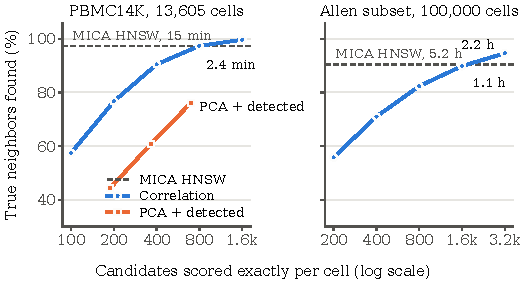
\includegraphics[width=\columnwidth]{figures/a2_neighbor_recall.pdf}
\caption{Share of each cell's 79 true MICA neighbors (the cell itself excluded) that a fast search recovers, checked by brute force on 500 random cells. Each curve shortlists candidates per cell, by correlation over all genes or by 50 principal components plus cells that share detected genes (for these, $x$ is the mean size of the merged list, and they were not run on the Allen subset). It then keeps the closest under the exact MICA distance. The dashed line is MICA's own HNSW search. Times are for building the full graph with 8 CPU workers.}
\label{fig:neighbors}
\end{figure}

\subsection{Neighbor search on subsets}
MICA's graph mode needs each cell's 80 nearest neighbors (itself included), and the HNSW search for them is its slowest step. To see whether a fast search misses important neighbors, we found the exact neighbors of 500 random cells by brute force (Fig.~\ref{fig:neighbors}). The ARIs here let the labels pick the setting, since they compare graphs, not selection rules.

On PBMC14K, shortlists from 50 principal components work poorly, finding 76\% of true neighbors at about 700 candidates per cell even with cells that share detected genes added. Correlation over all genes, one matrix product, does much better. With 800 candidates it finds 97.4\%, the same as MICA's HNSW (97.3\%), and building the graph for all cells took 2.4 minutes against 15 for HNSW. We then fed both graphs to MICA's own later steps (node2vec and Louvain). Our graph gave ARI 0.853 in two runs, and MICA's graph gave 0.852 twice.

On the 100,000 Allen cells, brute force for every cell would take about 43 hours. HNSW finds 90.3\% of true neighbors in 5.2 hours. Correlation finds 89.8\% with 1,600 candidates in 1.1 hours, and 94.6\% with 3,200 in 2.2 hours. These times use a faster exact distance that skips genes where the other cell sits in the lowest bin, and with the plain distance the 1,600 build would take about 2.3 hours. Through MICA's later steps, scored on the atlas's 34 cell classes, our 3,200 graph gives ARI 0.602 and 0.627 in two runs, against 0.617 and 0.641 for MICA's graph, and its AMI is about 0.01 lower each time.

The candidates needed grow with the data (800 at 13,605 cells, 1,600 at 100,000). Scaling the 100,000-cell pilot of MICA as shipped (7.1 hours, 140 GB) to 2.3 million cells gives 7 to 8 days and about 3.2 TB of memory, far above our 754 GB machine. So the full atlas needs a sketch (cluster a sample, then assign the rest), not only a faster search.

Hub cells also crowd the exact graph. On PBMC14K the top 1\% of cells fill 23\% of all exact neighbor slots, and their links join cells of the same type only 44\% of the time, against 75\% for other links. At the same resolution, Leiden partitions on our graph and on MICA's agree at ARI 0.98 on PBMC14K and 0.97 on the Allen subset.
